\chapter{TINJAUAN PUSTAKA}
\label{chap:tinjauanpustaka}

% Ubah bagian-bagian berikut dengan isi dari tinjauan pustaka

% Demi mendukung penelitian ini, \lipsum[1][1-5]

% \section{Roket Luar Angkasa}
% \label{sec:roketluarangkasa}

% % Contoh input gambar
% \begin{figure}[ht]
%   \centering

%   % Ubah dengan nama file gambar dan ukuran yang akan digunakan
%   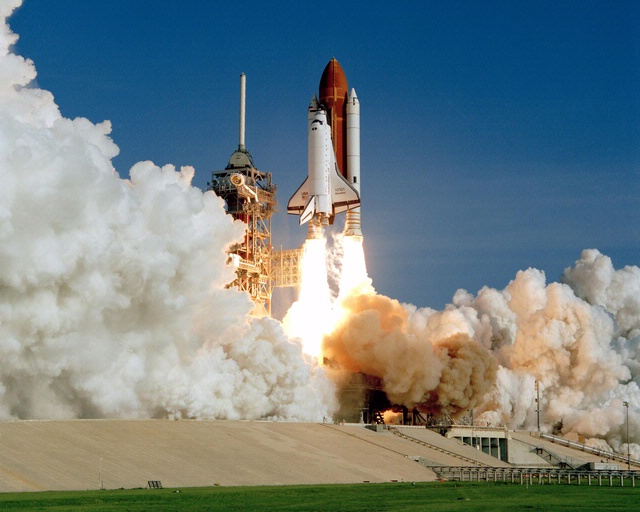
\includegraphics[scale=0.35]{gambar/roketluarangkasa.jpg}

%   % Ubah dengan keterangan gambar yang diinginkan
%   \caption{Peluncuran roket luar angkasa \emph{Discovery} \citep{roketluarangkasa}.}
%   \label{fig:roketluarangkasa}
% \end{figure}

% Roket luar angkasa merupakan \lipsum[1]

% \emph{Discovery}, Gambar \ref{fig:roketluarangkasa}, merupakan \lipsum[2]

\section{Deep Learning}
\label{sec:deeplearning}

Deep Learning sejatinya bagian machine learning yang dimana algoritma nya terinspirasi dari cara kerja jaringan neuron seperti halnya jaringan neuron pada otak manusia. Pada deep learning, syaraf atau neuron merupakan perwakilan dari satu fungsi yang menyimpan suatu nilai atau value yang dimana neuron - neuron ini berada dalam layer - layer yang dimana antar layer memiliki hubungan tertentu. Deep Learning digunakan karena kemampuanya untuk menemukan relasi yang tidak ditemukan antara input dan output. [5]

% \emph{Discovery}, Gambar \ref{fig:roketluarangkasa}, merupakan \lipsum[2]

\section{Convolutional Neural Network}
\label{sec:convolutionalneuralnetwork}

Convolutional Neural Network adalah metode deep learning yang didesain untuk rekognisi pada data dua dimensi yang dimana umumnya berupa gambar visual (tetapi tidak harus berupa gambar) dan untuk klasifikasi. Deep Learning dapat mengatasi masalah dimana terdapat terlalu banyak parameter.  Layer yang biasanya ada di dalam CNN yaitu input layer, convolutional layer, activation layer, dan fully connected layer.
Convolutional layer dan pooling layer merupakan bagian utama pada CNN. Layer - layer tersebut dapat menemukan karakteristik dari objek. Convolutional layer memiliki kapabilitas untuk menemukan dan meningkatkan fitur/karakteristik objek sedangkan pooling layer mampu menyaring fitur fitur yang ditemukan dengan menghapus layer yang tidak diperlukan atau meng-compress fitur. Activation layer memanfaatkan aktivasi non linear untuk meningkatkan expression ability dari model neural network. Fully Connected layer berfungsi untuk menggabungkan fitur - fitur objek dengan nilai output fitur. [6]

% \subsection{Hukum Newton}
% \label{subsec:hukumnewton}

% Newton \citep{newton1687} pernah merumuskan bahwa \lipsum[1]
% Kemudian menjadi persamaan seperti pada persamaan \ref{eq:hukumpertamanewton}.

% % Contoh pembuatan persamaan
% \begin{equation}
%   \label{eq:hukumpertamanewton}
%   \sum \mathbf{F} = 0\; \Leftrightarrow\; \frac{\mathrm{d} \mathbf{v} }{\mathrm{d}t} = 0.
% \end{equation}

% \subsection{Anti Gravitasi}
% \label{subsec:antigravitasi}

% Anti gravitasi merupakan \lipsum[1]


\section{Visi Komputer}
\label{sec:visikomputer}

Convolutional Neural Network adalah metode deep learning yang didesain untuk rekognisi pada data dua dimensi yang dimana umumnya berupa gambar visual (tetapi tidak harus berupa gambar) dan untuk klasifikasi. Deep Learning dapat mengatasi masalah dimana terdapat terlalu banyak parameter.  Layer yang biasanya ada di dalam CNN yaitu input layer, convolutional layer, activation layer, dan fully connected layer.
Convolutional layer dan pooling layer merupakan bagian utama pada CNN. Layer - layer tersebut dapat menemukan karakteristik dari objek. Convolutional layer memiliki kapabilitas untuk menemukan dan meningkatkan fitur/karakteristik objek sedangkan pooling layer mampu menyaring fitur fitur yang ditemukan dengan menghapus layer yang tidak diperlukan atau meng-compress fitur. Activation layer memanfaatkan aktivasi non linear untuk meningkatkan expression ability dari model neural network. Fully Connected layer berfungsi untuk menggabungkan fitur - fitur objek dengan nilai output fitur. [6]

\section{You Only Look Once (YOLO)}
\label{sec:youonlylookone}

You Only Look Once adalah algoritma yang memiliki kemampuan untuk mendeteksi dan mengenal objek yang ada di suatu gambar yang dimana hanya memerlukan satu propagasi di neural network. YOLO menggunakan CNN untuk melakukan deteksi objek secara real time. Dengan menggunakan YOLO berarti untuk melakukan deteksi pada suatu gambar hanya memerlukan sekali run .[6]

\section{Helm Keselamtan Kerja}
\label{sec:helmkeselamatankerja}

Helm Keselamatan Kerja atau yang kadang disebut Helm Proyek atau Hardhat  dalam bahasa inggris berfungsi sebagaimana helm pada umumnya berfungsi yaitu untuk melindungi kepala penggunanya. Berbeda dengan helm lainnya seperti helm motor atau helm militer, helm proyek digunakan umumnya pada proyek konstruksi untuk melindungi pekerja dari hantaman ke kepala saat terjatuh atau tertimpa benda berat yang dimana sering terjadi di wilayah konstruksi. [7]